\section{RepReMatch}

\subsection{Naïve Approach}
\begin{frame}{Naïve Approach}
	\begin{columns}[T, onlytextwidth]
		\begin{column}{0.55\textwidth}
			Greedy algorithm:
			\begin{itemize}
				\item<5->
				repeatedly use maximum weight matchings

				\item<6->
				fails because of missing foresight
				\begin{itemize}
					\item<7->
					\textsbf{additive valuations:}
					sort items by valuation \\
					\(\Rightarrow\) \(2n\)-approximation (\emph{SMatch})

					\item<8->
					\textsbf{submodular valuations:}
					lowest valuation \\
					approximable only by \(\bigomega[\big]{ \sqrt{m/\ln m} }\)
					\onslide<9->{\smash{\raisebox{-.25ex}{\textcolor{senfgelb}{\Large\Lightning}}}}
				\end{itemize}
			\end{itemize}
		\end{column}
		\begin{column}{0.45\textwidth}
			\vphantom{a}\vspace{-0.5\baselineskip}\par
			\centering
			\begin{tikzpicture}[val/.style = {font={\small\boldmath}, sloped, above}, match/.style = {}, match3/.style = {}]
				% Agents.
				\node<2-> at (0, 5) (a1) {
\includegraphics[height=8mm]{img/outstanding_agent}};
				\node<2-> at (0, 0) (a2) {
\includegraphics[height=8mm]{img/outstanding_agent}};

				% Items (first batch).
				\node<2-3|handout:0> at (       4, 5) (i1) {
\includegraphics[height=6mm]{img/naive_item}};
				\node<2-3|handout:0> at (       4, 0) (i6) {
\includegraphics[height=6mm]{img/naive_item}};
				\node<4- |handout:1> at (-0.65, 5)      {
\includegraphics[height=6mm]{img/naive_item}};
				\node<4- |handout:1> at (-0.65, 0)      {
\includegraphics[height=6mm]{img/naive_item}};

				% Edges (first batch).
				\only<3|handout:0>{\tikzset{match/.style={alert}}}

				\draw<2-3|handout:0>        (a2.east) -- node[val, pos=0.25] {\(\weight[2] \cdot \symup{log}~ \valuations[\genericitem[1]][\big][2]\)} (i1.west);
				\draw<2-3|handout:0>        (a1.east) -- node[val, pos=0.25] {\(\weight[1] \cdot \symup{log}~ \valuations[\genericitem[2]][\big][1]\)} (i6.west);
				\draw<2-3|handout:0>[match] (a1.east) -- node[val]           {\(\weight[1] \cdot \symup{log}~ \valuations[\genericitem[1]][\big][1]\)} (i1.west);
				\draw<2-3|handout:0>[match] (a2.east) -- node[val]           {\(\weight[2] \cdot \symup{log}~ \valuations[\genericitem[2]][\big][2]\)} (i6.west);

				% Items (third batch)
				\node<5-8|handout:1> at ( 4.00, 1) (i5) {
\includegraphics[height=6mm]{img/naive_item}};
				\node<5-8|handout:1> at ( 4.00, 3) (i3) {
\includegraphics[height=6mm]{img/naive_item}};
				\node<9- |handout:0> at (-1.95, 5) (i5) {
\includegraphics[height=6mm]{img/naive_item}};
				\node<9- |handout:0> at (-1.95, 0) (i3) {
\includegraphics[height=6mm]{img/naive_item}};

				% Edges (third batch)
				\only<8|handout:0>{\tikzset{match3/.style={alert}}}

				\draw<5-8|handout:1>         (a2.east) -- (i3.west);
				\draw<5-8|handout:1>         (a1.east) -- (i5.west);
				\draw<5-8|handout:1>[match3] (a1.east) -- (i3.west);
				\draw<5-8|handout:1>[match3] (a2.east) -- (i5.west);

				% Items (second batch)
				\node<5-6|handout:1> at (   4, 4) (i2) {
\includegraphics[height=6mm]{img/naive_item}};
				\node<5-6|handout:1> at (   4, 2) (i4) {
\includegraphics[height=6mm]{img/naive_item}};
				\node<7- |handout:0> at (-1.3, 5)      {
\includegraphics[height=6mm]{img/naive_item}};
				\node<7- |handout:0> at (-1.3, 0)      {
\includegraphics[height=6mm]{img/naive_item}};

				% Edges (second batch)
				\only<6|handout:1>{\tikzset{match/.style={alert}}}

				\draw<5-6|handout:1>        (a1.east) -- (i2.west);
				\draw<5-6|handout:1>        (a2.east) -- (i4.west);
				\draw<5-6|handout:1>[match] (a2.east) -- (i2.west);
				\draw<5-6|handout:1>[match] (a1.east) -- (i4.west);

				% Dilators.
				\node<2->[opacity=0] at (-1.950, 5)       {
\includegraphics[height=6mm]{img/naive_item}};
				\node<2->[opacity=0] at (-1.30, 5)       {
\includegraphics[height=6mm]{img/naive_item}};
				\node<2->[opacity=0] at (-0.65, 5)       {
\includegraphics[height=6mm]{img/naive_item}};
				\node<2->[opacity=0] at ( 4.00, 5) (inv) {
\includegraphics[height=6mm]{img/naive_item}};

				\draw<2->[opacity=0] (a1.east) -- node[val, pos=0.25] {\(\weight[2] \cdot \symup{log}~ \valuations[\genericitem[1]][\big][2]\)} (inv.west);
			\end{tikzpicture}
		\end{column}
	\end{columns}
\end{frame}





\subsection{The Algorithm}
\begin{frame}{Key Ideas of the Algorithm}
	\begin{columns}[t, onlytextwidth]
		\begin{column}{0.6\textwidth}
			We need change the past in three phases:
			\begin{description}
				\item[Phase \phasei]
				Assign enough high-value items temporarily.

				\item[Phase \phaseii]
				Assign the remaining items definitely.

				\item[Phase \phaseiii]
				Re-assign the items of phase \phasei{} definitely.
			\end{description}

			\smallskip

			\begin{exampleblock}{Theorem}
				RepReMatch guarantees a \(2n(\log_2 n + 3)\)-approximation \\
				under submodular valuations.
			\end{exampleblock}
		\end{column}
		\begin{column}{0.4\textwidth}
			\vphantom{a}\vspace{-0.5\baselineskip}\par
			\centering
			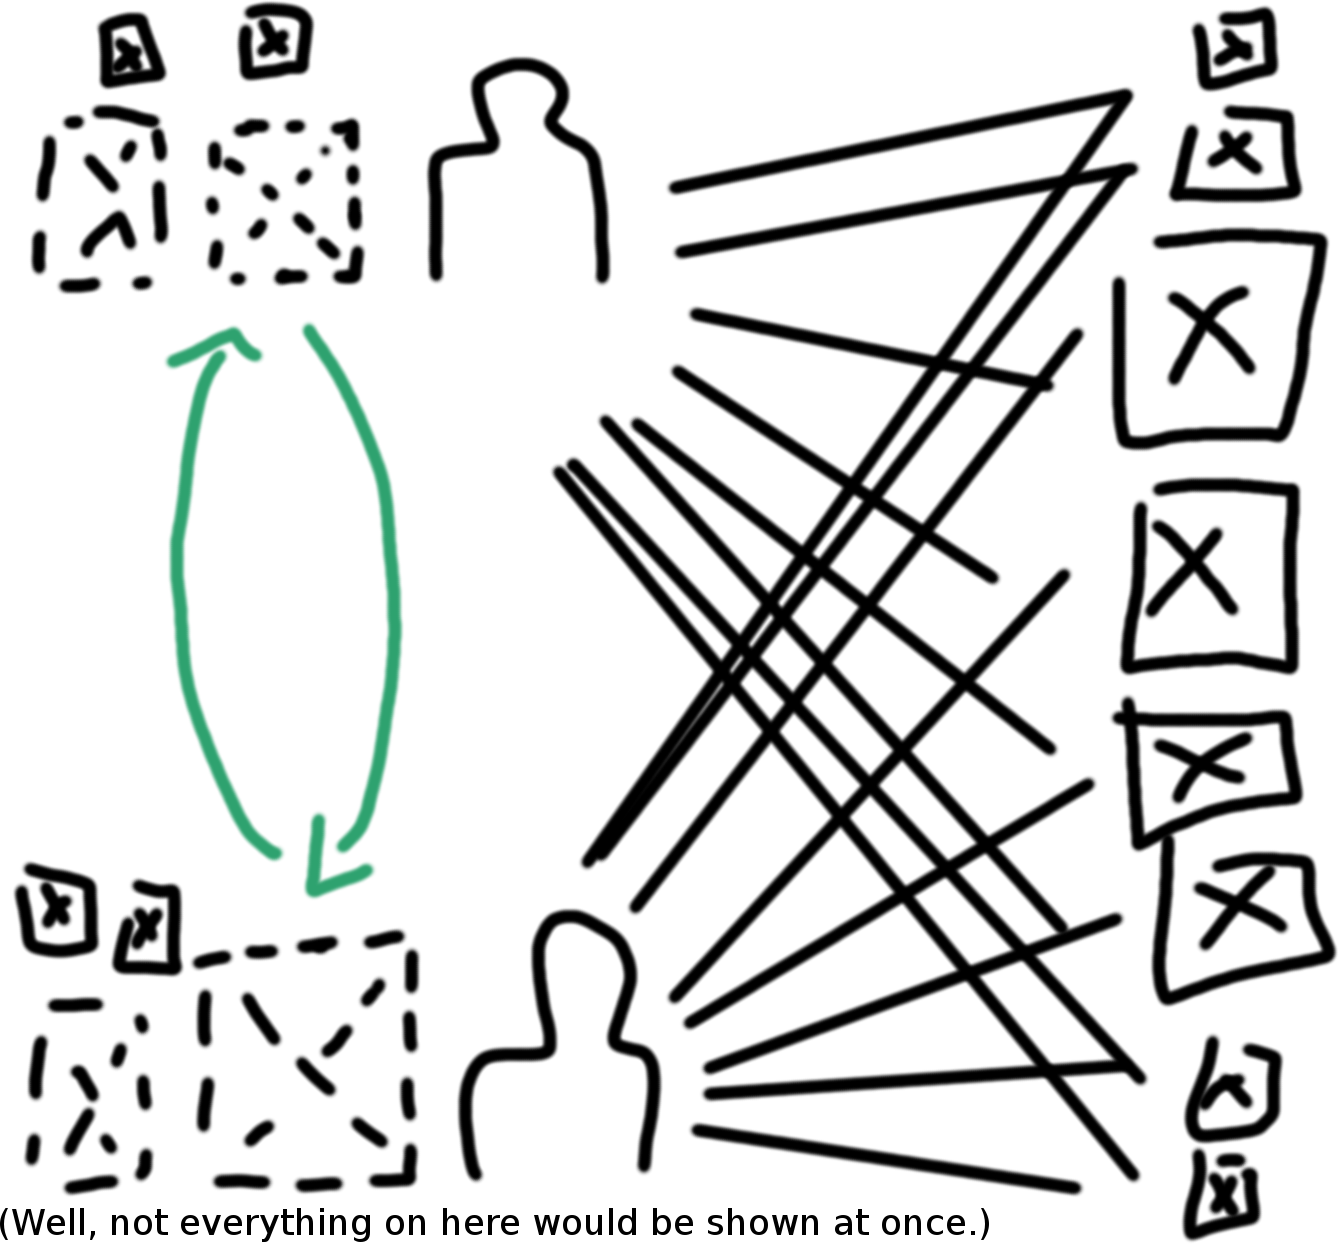
\includegraphics[height=5cm]{img/phases}
		\end{column}
	\end{columns}
\end{frame}

\begin{frame}{The Algorithm}
	\pause
	\onslide<+->{Phase \phasei:}
	\begin{enumerate}[<+->]
		\item
		repeat \(\ceil{\log_2 n} + 1\) times
		\begin{enumerate}[<+->]
			\item
			create bipartite graph \((\agents, \goods, E)\) with edge weights \(\log \valuations[ \hairspace j ]^{\weight}\)

			\item
			compute maximum weight matching

			\item
			update bundles \(\alloc[\phasei]\) \& remove assigned items
		\end{enumerate}
		\seti
	\end{enumerate}
	\onslide<+->{Phase \phaseii:}
	\begin{enumerate}[<+->]
		\conti
		\item
		repeat until \(\goods = \emptyset\)
		\begin{enumerate}[<+->]
			\item
			create bipartite graph \((\agents, \goods, E)\) with edge weights \(\log \valuations[\alloc[\phaseii] \cup \{ \hairspace j \} ]^{\weight} \)

			\item
			compute maximum weight matching

			\item
			update bundles \(\alloc[\phaseii]\) \& remove assigned items
		\end{enumerate}
		\seti
	\end{enumerate}
	\onslide<+->{Phase \phaseiii:}
	\begin{enumerate}[<+->]
		\conti
		\item
		create bipartite graph \(\paren[\big]{ \agents, \bigcup_{i \in \agents} \alloc[\phasei], E }\) with edge weights \(\log \valuations[\alloc[\phaseii] \cup \{ \hairspace j \} ]^{\weight} \)

		\item
		compute maximum weight matching

		\item
		create bundles \(\alloc[\phaseiii]\)
	\end{enumerate}
\end{frame}





\subsection{Analysing Phases \texorpdfstring{\phasei{} \& \phaseiii}{I \& III}}
\begin{frame}{Analysing Phases \phasei{} \& \phaseiii{} (1/2)}
	\pause
	\onslide<+->{Phase \phasei{} reserves \enquote{high-value} items.}
	\onslide<+->{But what qualifies as \enquote{high-value}?}

	\begin{definition}<+->
		Let \(\alloc* = \braces[\big]{ \asgd*{1}, \asgd*{2}, \dots }\) be an optimal bundle.
		\onslide<+->{An item \(\genericitem \in \goods\) is \emph{outstanding} if \(\valuations[ \hairspace \genericitem] \ge \valuations[\asgd*{1}][\big]\).}
	\end{definition}

	\onslide<+->{\(\Rightarrow\) Are enough outstanding items reserved?}
\end{frame}

\begin{frame}{Analysing Phases \phasei{} \& \phaseiii{} (2/2)}
	\adjustfortopblock
	\begin{lemma}
		Each agent can be matched with an outstanding item in phase \phaseiii.
	\end{lemma}
	\begin{columns}[T]
		\begin{column}{0.6\textwidth}
			\begin{itemize}[<+(1)->]
				\item
				maximum number of unmatched agents halved \\
				with each round of phase \phasei
				\begin{itemize}[<+(1)->]
					\item
					\(\ceil{\log_2 n} + 1\) rounds in phase \phasei{} are enough
				\end{itemize}

				\item
				induction on number of rounds in phase \phasei
			\end{itemize}
			\onslide<+(1)->{Base Case: In round \(1\) of phase \phasei, either}
			\begin{itemize}[<+(1)->]
				\item
				\(\ge n/2\) many agents matched with an outstanding item

				\item
				\(< n/2\) many agents matched with an outstanding item
				\begin{itemize}
					\item<+(1)->
					\(> n/2\) many items \(\asgd*{1}\) assigned to someone else

					\item<+(5)->
					\(> n/2\) many agents matched upon release in phase \phaseiii
				\end{itemize}
			\end{itemize}
		\end{column}
		\begin{column}{0.375\textwidth}
			\centering
			\begin{tikzpicture}[lbl/.style = {font={\Large\boldmath}}]
				% Agents.
				\node<5->[lbl] at (0, 4) (a1) {
\includegraphics[height=8mm]{img/outstanding_agent}\hspace{-4.05mm}\(1\)};
				\node<5->[lbl] at (0, 3) (a2) {
\includegraphics[height=8mm]{img/outstanding_agent}\hspace{-4.05mm}\(2\)};
				\node<5->[lbl] at (0, 2) (a3) {
\includegraphics[height=8mm]{img/outstanding_agent}\hspace{-4.05mm}\(3\)};
				\node<5->[lbl] at (0, 1) (a4) {
\includegraphics[height=8mm]{img/outstanding_agent}\hspace{-4.05mm}\(4\)};
				\node<5->[lbl] at (0, 0) (a5) {
\includegraphics[height=8mm]{img/outstanding_agent}\hspace{-4.05mm}\(5\)};

				% Items (outlines).
				\node<5-> at (3, 4) (i1) {
\includegraphics[height=8mm]{img/outstanding_item}};
				\node<5-> at (3, 3) (i2) {
\includegraphics[height=8mm]{img/outstanding_item}};
				\node<5-> at (3, 2) (i3) {
\includegraphics[height=8mm]{img/outstanding_item}};
				\node<5-> at (3, 1) (i4) {
\includegraphics[height=8mm]{img/outstanding_item}};
				\node<5-> at (3, 0) (i5) {
\includegraphics[height=8mm]{img/outstanding_item}};

				% Edges.
				\def\xoffset{++(5.5mm,0)}
				\draw< 5-12>  % phase I
					(a1)\xoffset -- (i1)
					(a2)\xoffset -- (i2)
					(a3)\xoffset -- (i3)
					(a4)\xoffset -- (i4)
					(a5)\xoffset -- (i5)
				;
				\draw<13-  >  % phase III
					(a1)\xoffset -- (i4.west)
					(a2)\xoffset -- (i5.west)
					(a3)\xoffset -- (i1.west)
					(a4)\xoffset -- (i3.west)
					(a5)\xoffset -- (i2.west)
				;

				% Items (planks).
				\node<5- 9> at (3, 4) {
\includegraphics[height=8mm]{img/outstanding_itemplanks}};
				\node<5-11> at (3, 3) {
\includegraphics[height=8mm]{img/outstanding_itemplanks}};
				\node<5-10> at (3, 2) {
\includegraphics[height=8mm]{img/outstanding_itemplanks}};
				\node<5- 8> at (3, 1) {
\includegraphics[height=8mm]{img/outstanding_itemplanks}};
				\node<5-  > at (3, 0) {
\includegraphics[height=8mm]{img/outstanding_itemplanks}};

				% Ticks and crosses (dilator).
				\node<-5>[opacity=0] at (-.25, 4) {
\includegraphics[height=8mm]{img/outstanding_tick}};

				% Ticks and crosses (case 1).
				\node<6> at (-.25, 4) {
\includegraphics[height=8mm]{img/outstanding_tick}};
				\node<6> at (-.25, 3) {
\includegraphics[height=8mm]{img/outstanding_tick}};
				\node<6> at (-.25, 2) {
\includegraphics[height=8mm]{img/outstanding_cross}};
				\node<6> at (-.25, 1) {
\includegraphics[height=8mm]{img/outstanding_tick}};
				\node<6> at (-.25, 0) {
\includegraphics[height=8mm]{img/outstanding_tick}};

				% Ticks and crosses (case 2 (bad)).
				\node<7-12> at (-.25, 4) {
\includegraphics[height=8mm]{img/outstanding_cross}};
				\node<7-12> at (-.25, 3) {
\includegraphics[height=8mm]{img/outstanding_tick}};
				\node<7-12> at (-.25, 2) {
\includegraphics[height=8mm]{img/outstanding_cross}};
				\node<7-12> at (-.25, 1) {
\includegraphics[height=8mm]{img/outstanding_cross}};
				\node<7-12> at (-.25, 0) {
\includegraphics[height=8mm]{img/outstanding_cross}};

				% Items (labels).
				\node<10->[lbl] at (3, 4) {\(\asgd*{1}[3]\)};
				\node<12->[lbl] at (3, 3) {\(\asgd*{1}[5]\)};
				\node<11->[lbl] at (3, 2) {\(\asgd*{1}[4]\)};
				\node< 9->[lbl] at (3, 1) {\(\asgd*{1}[1]\)};

				% Ticks and crosses (case 2 (good)).
				\node<13-> at (-.25, 4) {
\includegraphics[height=8mm]{img/outstanding_tick}};
				\node<13-> at (-.25, 3) {
\includegraphics[height=8mm]{img/outstanding_cross}};
				\node<13-> at (-.25, 2) {
\includegraphics[height=8mm]{img/outstanding_tick}};
				\node<13-> at (-.25, 1) {
\includegraphics[height=8mm]{img/outstanding_tick}};
				\node<13-> at (-.25, 0) {
\includegraphics[height=8mm]{img/outstanding_tick}};
			\end{tikzpicture}
		\end{column}
	\end{columns}
\end{frame}





\subsection{Analysing Phase \texorpdfstring{\phaseii}{II}}
\begin{frame}[fragile]{Analysing Phase \phaseii{} (1/2)}
	\adjustfortopblockincolumn
	\begin{columns}[t, onlytextwidth]
		\begin{column}{0.55\textwidth}
			\begin{definition}<2->
				The set \(\lostset{r}\) of \emph{lost items} is the set of all optimal items \(j \in \alloc*\)
				\onslide<3->{matched with other agents \(i' \neq i\) in round \(r\).}
			\end{definition}
			\begin{definition}<4->
				Let \(\alloc[\phaseii] = \braces[\big]{ \asgd{1}, \asgd{2}, \dots }\) be the bundle of agent \(i\).
				\onslide<5->{The set of \emph{optimal and attainable items} is defined as
				\begin{equation*}
					\attopt{r} \coloneq \begin{cases*}
						\onslide*<-10>{\phantom}{\alloc* \setminus \paren[\big]{ \bigcup_{i' \in \agents} \alloc[\phasei][i'] \cup \lostset{1} }}
						& \onslide*<-5>{\phantom}{in round \(r = 1\), } \\
						\onslide*<-18>{\phantom}{ \attopt{r-1} \setminus \paren[\big]{ \lostset{r} \cup \braces[\big]{ \asgd{r-1} } } }
						& \onslide*<-11>{\phantom}{in round \(r \ge 2\).}
					\end{cases*}
				\end{equation*}}
			\end{definition}

			\onslide<20->{\(\Rightarrow\) What is the valuation of the remaining items?}
		\end{column}
		\begin{column}{0.45\textwidth}
			\begin{figure}
				\begin{tikzpicture}
					\node< 7- 9> {\includegraphics[height=25mm]{optainable_r1_optblack}};
					\node<10-  > {\includegraphics[height=25mm]{optainable_r1_optgrey}};
					\node< 8-  > {\includegraphics[height=25mm]{optainable_r1_phIfill}};
					\node< 7-  > {\includegraphics[height=25mm]{optainable_r1_optoutline}};
					\node< 8-  > {\includegraphics[height=25mm]{optainable_r1_phIoutline}};
					\node< 9-  > {\includegraphics[height=25mm]{optainable_r1_lost}};

					\node< 7->[legend            ] at (-2.00,  0.50) {\(\alloc*\)};
					\node< 8->[legend, emorot    ] at ( 2.00,  0.65) {\(\bigcup_{i' \in \agents} \alloc[\phasei][i']\)};
					\node< 9->[legend, goetheblau] at (-0.65,  0.25) {\(\lostset{1}\)};
					\node<10->[legend, dunkelgrau] at (-0.30, -0.75) {\(\attopt{1}\)};
				\end{tikzpicture}

				\vspace{2ex}

				\let\asgd\asgdbf
				\begin{tikzpicture}
					\node<13-17> {\includegraphics[height=25mm]{optainable_r2_optblack}};
					\node<18-  > {\includegraphics[height=25mm]{optainable_r2_optgrey}};
					\node<14-  > {\includegraphics[height=25mm]{optainable_r2_lost}};
					\node<16-  > {\includegraphics[height=25mm]{optainable_r2_asgdleft}};
					\node<17-  > {\includegraphics[height=25mm]{optainable_r2_asgdright}};
					\node<18-  > {\includegraphics[height=25mm]{optainable_r2_optoverlay}};

					\node<13->[legend             ] at (-2.15,  0.75) {\(\attopt{r-1}\)};
					\node<14->[legend, goetheblau ] at ( 1.75, -0.65) {\(\lostset{r}\)};
					\node<15->[legend, dunkelgruen] at ( 1.67,  1.00) {\(\asgd{r-1}\)};
					\node<16->[legend, dunkelgruen] at ( 0.36,  0.35) {\(?\)};
					\node<17->[legend, dunkelgruen] at ( 2.35,  0.35) {\(?\)};
					\node<18->[legend, dunkelgrau ] at (-0.75, -0.25) {\(\attopt{r}\)};
				\end{tikzpicture}
			\end{figure}
		\end{column}
	\end{columns}
\end{frame}

\begin{frame}{Analysing Phase \phaseii{} (2/2)}
	\adjustfortopblock
	\begin{lemma}
		\vspace{-3ex}
		\begin{flalign*}
			\valuations[ \attopt{r} \given \asgd{1}, \dots, \asgd{r-1} ][\big]
			\temporal<18-23>{}{=}{\ge}
			\onslide*<18-19>{\valuations[ \attopt{r} \cup \braces[\big]{\asgd{1}, \dots, \asgd{r-1}} ][\big] \alertmath<19>{{} - \valuations[\asgd{1}, \dots, \asgd{r-1}][\big]}}
			\onslide*<20-  >{\alertmath<20>{- \valuations[\asgd{1}, \dots, \asgd{r-1}][\big]} +}
			\onslide*<20-23>{\alertmath<21-23>{\valuations[ \attopt{r} \cup \braces[\big]{\asgd{1}, \dots, \asgd{r-1}} ][\big]}}
			\onslide*<24-  >{\valuations[ \attopt{1} ][\big]}
			\onslide*<25-27>{- \valuations[ \lostset{2} \given \asgd{1} ][\big]}
			\onslide*<26-27>{- \valuations[ \lostset{3} \given \asgd{1}, \asgd{2} ][\big]}
			\onslide*<27   >{- \dots}
			\onslide*<28-36>{- \!\!\sum_{l=2}^{r} \valuations[ \lostset{l} \given \asgd{1}, \dots, \asgd{l-1} ][\big] }
			\onslide*<37-39>{- \!\!\sum_{l=2}^{r} \smashoperator[r]{\sum_{\genericitem \in \lostset{l}}} \valuations[ \hairspace\genericitem \given \asgd{1}, \dots, \alertmath<39>{\asgd{l-1}} ][\big] }
			\onslide*<40-41>{- \!\!\sum_{l=2}^{r} \smashoperator[r]{\sum_{\genericitem \in \lostset{l}}} \valuations[ \hairspace\genericitem \given \asgd{1}, \dots, \alertmath<40>{\asgd{l-2}} ][\big] }
			\onslide*<42   >{- \!\!\sum_{l=2}^{r} \smashoperator[r]{\sum_{\genericitem \in \lostset{l}}} \valuations[ \asgd{l-1} \given \asgd{1}, \dots, \asgd{l-2} ][\big] }
			\onslide*<43   >{- \!\!\sum_{l=2}^{r} \abs{\lostset{l}} \cdot \valuations[ \asgd{l-1} \given \asgd{1}, \dots, \asgd{l-2} ][\big] }
			\onslide*<44   >{- \!\!\sum_{l=2}^{r} (n-1) \cdot \valuations[ \asgd{l-1} \given \asgd{1}, \dots, \asgd{l-2} ][\big] }
			\vphantom{\sum_{\genericitem \in \lostset{l}}^{r}}&&
		\end{flalign*}
	\end{lemma}
	\vspace{-1ex}
	\begin{figure}
		\hspace{-3em}
		\begin{tikzpicture}
			\node< 1   >[opacity=0] {\includegraphics[height=45mm]{optainable_anal_asgdf_1}};  % prevents wobbling of lemma block in otherwise empty page
			\node< 2-  > {\includegraphics[height=45mm]{optainable_anal_optblack}};
			\node<17-  > {\includegraphics[height=45mm]{optainable_anal_optgrey}};
			\node< 3- 4> {\includegraphics[height=45mm]{optainable_anal_asgdf_1}};
			\node< 5- 6> {\includegraphics[height=45mm]{optainable_anal_asgdf_2}};
			\node< 7- 8> {\includegraphics[height=45mm]{optainable_anal_asgdf_3}};
			\node< 9-10> {\includegraphics[height=45mm]{optainable_anal_asgdf_4}};
			\node<11-12> {\includegraphics[height=45mm]{optainable_anal_asgdf_5}};
			\node<13-14> {\includegraphics[height=45mm]{optainable_anal_asgdf_6}};
			\node<15-  > {\includegraphics[height=45mm]{optainable_anal_asgdf_7}};
			\node< 2-  > {\includegraphics[height=45mm]{optainable_anal_optoutline}};
			\node< 3- 4> {\includegraphics[height=45mm]{optainable_anal_asgdl_1}};
			\node< 5- 6> {\includegraphics[height=45mm]{optainable_anal_asgdl_2}};
			\node< 7- 8> {\includegraphics[height=45mm]{optainable_anal_asgdl_3}};
			\node< 9-10> {\includegraphics[height=45mm]{optainable_anal_asgdl_4}};
			\node<11-12> {\includegraphics[height=45mm]{optainable_anal_asgdl_5}};
			\node<13-14> {\includegraphics[height=45mm]{optainable_anal_asgdl_6}};
			\node<15-  > {\includegraphics[height=45mm]{optainable_anal_asgdl_7}};
			\node< 4-  > {\includegraphics[height=45mm]{optainable_anal_lost_1}};
			\node< 6-  > {\includegraphics[height=45mm]{optainable_anal_lost_2}};
			\node< 8-  > {\includegraphics[height=45mm]{optainable_anal_lost_3}};
			\node<10-  > {\includegraphics[height=45mm]{optainable_anal_lost_4}};
			\node<12-  > {\includegraphics[height=45mm]{optainable_anal_lost_5}};
			\node<14-  > {\includegraphics[height=45mm]{optainable_anal_lost_6}};
			\node<16-  > {\includegraphics[height=45mm]{optainable_anal_lost_7}};
			\node<22   > {\includegraphics[height=45mm]{optainable_anal_emph_big}};
			\node<23   > {\includegraphics[height=45mm]{optainable_anal_emph_small}};

			\node< 2->[legend             ] at (-3.25,  0.50) {\(\attopt{1}\)};
			\node< 3->[legend, dunkelgruen] at ( 2.50, -1.75) {\(\alloc[\phaseii]\)};
			\node< 4->[legend, goetheblau ] at ( 3.57,  0.20) {\(\lostset{\cdot}\)};
			\node<17->[legend, dunkelgrau ] at (-1.00,  0.10) {\(\attopt{r}\)};
		\end{tikzpicture}
	\end{figure}
	\onslide*<29-37>{\beamerimage at (13cm, 3.25cm) {%
		\begin{minipage}[t][5cm]{0.4\textwidth}\begin{flalign*}
			\valuations[ \genericset[1] \given \genericset[2] ] \alt<35->{\le {}}{= {}}
			\onslide*<30-34>{&\valuations[\hairspace\genericitem[1] \given \genericset[2] ][\big]}
			\onslide*<31-34>{{} + {} \\ &\valuations[\hairspace\genericitem[2] \given \genericset[2] \cup \alertmath<34>{\braces[\big]{ \genericitem[1] }} ][\big]}
			\onslide*<32-34>{{} + {} \\ &\valuations[\hairspace\genericitem[3] \given \genericset[2] \cup \alertmath<34>{\braces[\big]{ \genericitem[1], \genericitem[2] }} ][\big]}
			\onslide*<33-34>{{} + {} \\ &\vdots}
			\onslide*<35   >{&\valuations[ \hairspace\genericitem[1] \given \genericset[2] ][\big] + {} \\ &\valuations[ \hairspace\genericitem[2] \given \genericset[2] ][\big] + {} \\ &\valuations[ \hairspace\genericitem[3] \given \genericset[2] ][\big] + {} \\ &\vdots}
			\onslide*<36-  >{\!\!\smashoperator{\sum_{\genericitem \in \genericset[1]}} \valuations[ \hairspace\genericitem  \given \genericset[2] ] }
			&&
		\end{flalign*}\end{minipage}
	};}
\end{frame}